\documentclass{standalone}
\usepackage{tikz}

\begin{document}

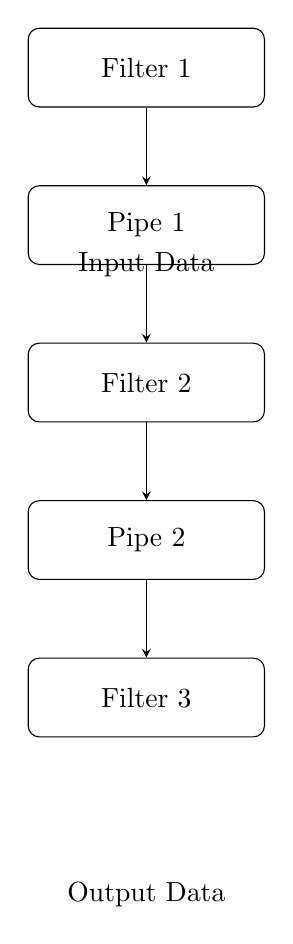
\begin{tikzpicture}[node distance=2cm]
    % Define styles for nodes
    \tikzstyle{box} = [rectangle, draw=black, fill=white, text centered, rounded corners, minimum width=3cm, minimum height=1cm]

    % Create nodes (pipes and filters)
    \node (filter1) [box] {Filter 1};
    \node (pipe1) [box, below of=filter1] {Pipe 1};
    \node (filter2) [box, below of=pipe1] {Filter 2};
    \node (pipe2) [box, below of=filter2] {Pipe 2};
    \node (filter3) [box, below of=pipe2] {Filter 3};

    % Draw connections between nodes
    \draw[-stealth] (filter1.south) -- (pipe1.north);
    \draw[-stealth] (pipe1.south) -- (filter2.north);
    \draw[-stealth] (filter2.south) -- (pipe2.north);
    \draw[-stealth] (pipe2.south) -- (filter3.north);

    % Add labels to indicate the direction of data flow
    \node[below of=filter1, yshift=-0.5cm] {Input Data};
    \node[below of=filter3, yshift=-0.5cm] {Output Data};
\end{tikzpicture}

\end{document}